\documentclass[a4paper,14pt]{article}

\usepackage{comment} % Para comentar várias linhas ao mesmo tempo

%matemática
\usepackage{amsmath}
\usepackage{amssymb}

%diagramação
\usepackage{extsizes}
\everymath{\displaystyle}
\usepackage{geometry}
\usepackage{fancyhdr}
\usepackage{multicol}
\usepackage{graphicx}
\usepackage[brazil]{babel}
\usepackage[shortlabels]{enumitem}
\usepackage{cancel}
\usepackage{textcomp}
\usepackage{tcolorbox}

%tabelas
\usepackage{array} % Para melhor formatação de tabelas
\usepackage{longtable}
\usepackage{booktabs}  % Para linhas horizontais mais bonitas
\usepackage{float}   % Para usar o modificador [H]
\usepackage{caption} % Para usar legendas em tabelas
\usepackage{wrapfig} % Para usar tabelas e figuras flutuantes


%tikzpicture
\usepackage{tikz}
\usepackage{scalerel}
\usepackage{pict2e}
\usepackage{tkz-euclide}
\usetikzlibrary{calc}
\usetikzlibrary{patterns,arrows.meta}
\usetikzlibrary{shadows}
\usetikzlibrary{external}

%pgfplots
\usepackage{pgfplots}
\pgfplotsset{compat=newest}
\usepgfplotslibrary{statistics}
\usepgfplotslibrary{fillbetween}

%colours
\usepackage{xcolor}



\columnsep=2cm
\hoffset=0cm
\textwidth=8cm
\setlength{\columnseprule}{.1pt}
\setlength{\columnsep}{2cm}
\renewcommand{\headrulewidth}{0pt}
\geometry{top=1in, bottom=1in, left=0.7in, right=0.5in}

\pagestyle{fancy}
\fancyhf{}
\fancyfoot[C]{\thepage}

\begin{document}
	
	\noindent\textbf{6FMA79 - Matemática} 
	
	\begin{center}Revisão: introdução aos números inteiros - Oposto, ordem e módulo (Versão estudante)
	\end{center}
	
	\noindent\textbf{Nome:} \underline{\hspace{10cm}}
	\noindent\textbf{Data:} \underline{\hspace{4cm}}
	
	%\section*{Questões de Matemática}
	
	\begin{multicols}{2}
		\noindent
		\begin{itemize}
			\item O oposto (ou simétrico) de um número inteiro $x$ é o número que está à mesma distância de $x$ ao zero, mas em sentido oposto. Indicamos o oposto de $x$ por $-x$.
			\item Representando os números inteiros na reta cujo sentido é da esquerda para a direita, se um número $a$ está à direita de um número $b$ diremos que $a$ é maior que $b$ ou que $b$ é menor que $a$ e indicamos $a > b$ ou $b < a$.
			\item O módulo ou valor absoluto de um número inteiro $x$ é a distância de zero até o número $x$. Indicamos o módulo de $x$ por $|x|$.
		\end{itemize}
		\noindent\textsubscript{-----------------------------------------------------------------------}
    	\begin{enumerate}
   			\item Veja as ilustrações e diga quanto vale $x$ e quanto vale $-x$. Observe o sentido dos eixos.
			\begin{enumerate}[a)]
				\item ~\\ \begin{tikzpicture}
					 % Desenha a reta
					\draw[thick] (0,0) -- (6.5,0); % Reta horizontal de (0,0) a (9,0)
					% Desenha os círculos nos pontos da reta
					\foreach \x in {0.66, 1.33, 1.98, 2.64, 3.33, 3.96, 4.62, 5.28, 5.94} { % Para cada ponto em {1, 2, 3, 4, 5, 6, 7, 8, 9}
					\fill (\x, 0) circle (3pt); % Desenha um círculo de raio 3pt em (x, 0)
					% Adiciona legendas nos pontos específicos
					\node at (1.33, -0.4) {x};   % Legenda "x" no segundo ponto
					\node at (3.33, -0.4) {0};    % Legenda "0" no quinto ponto
					\node at (3.96, -0.4) {1};    % Legenda "1" no sexto ponto
				}
				\end{tikzpicture} 
				\item ~\\ \begin{tikzpicture}
					% Desenha a reta
					\draw[thick] (0,0) -- (6.5,0); % Reta horizontal de (0,0) a (9,0)
					% Desenha os círculos nos pontos da reta
					\foreach \x in {0.66, 1.33, 1.98, 2.64, 3.33, 3.96, 4.62, 5.28, 5.94} { % Para cada ponto em {1, 2, 3, 4, 5, 6, 7, 8, 9}
						\fill (\x, 0) circle (3pt); % Desenha um círculo de raio 3pt em (x, 0)
						% Adiciona legendas nos pontos específicos
						\node at (2.64, -0.4) {-x};   % Legenda "x" no quarto ponto
						\node at (5.94, -0.4) {0};    % Legenda "0" no nono ponto
					}
				\end{tikzpicture}
				\item ~\\ \begin{tikzpicture}
					% Desenha a reta
					\draw[thick] (0,0) -- (6.5,0); % Reta horizontal de (0,0) a (9,0)
					% Desenha os círculos nos pontos da reta
					\foreach \x in {0.66, 1.33, 1.98, 2.64, 3.33, 3.96, 4.62, 5.28, 5.94} { % Para cada ponto em {1, 2, 3, 4, 5, 6, 7, 8, 9}
						\fill (\x, 0) circle (3pt); % Desenha um círculo de raio 3pt em (x, 0)
						% Adiciona legendas nos pontos específicos
						\node at (1.33, -0.4) {-2};   % Legenda "-2" no segundo ponto
						\node at (5.28, -0.4) {x};    % Legenda "x" no oitavo ponto
					}
				\end{tikzpicture}
				\item ~\\ \begin{tikzpicture}
					% Desenha a reta
					\draw[thick] (0,0) -- (6.5,0); % Reta horizontal de (0,0) a (9,0)
					% Desenha os círculos nos pontos da reta
					\foreach \x in {0.66, 1.33, 1.98, 2.64, 3.33, 3.96, 4.62, 5.28, 5.94} { % Para cada ponto em {1, 2, 3, 4, 5, 6, 7, 8, 9}
						\fill (\x, 0) circle (3pt); % Desenha um círculo de raio 3pt em (x, 0)
						% Adiciona legendas nos pontos específicos
						\node at (1.33, -0.4) {-3};   % Legenda "-2" no segundo ponto
						\node at (3.33, -0.4) {-x};    % Legenda "x" no quinto ponto
						\node at (5.94, -0.4) {4};    % Legenda "4" no nono ponto
					}
				\end{tikzpicture}
			\end{enumerate}			
			\item Assinale \textbf{V} (verdadeiro) ou \textbf{F} (falso).
			\begin{enumerate}[a)]
				\item (~~) Se $x$ é um número inteiro, então $-x$ é negativo.
				\item (~~) O oposto do simétrico de -7 é 7.
				\item (~~) O simétrico de $-x$ é $x$, para todo $x$ inteiro.
				\item (~~) Não existe $x$ inteiro igual ao seu oposto.
			\end{enumerate}
			\item Assinale \textbf{V} (verdadeiro) ou \textbf{F} (falso).
			\begin{enumerate}[a)]
				\item (~~) $12 < 15$
				\item (~~) $21 \leq 21$
				\item (~~) $-3 > -5 \leq 0$
				\item (~~) $-4 < -2 < 2$
				\item (~~) $-x < x$ para todo $x$ inteiro.
				\item (~~) Todo número inteiro negativo é menor que qualquer número inteiro positivo.
			\end{enumerate}
			\item Dado $x \in \mathbb{Z}$, defina $|x|$, isto é, diga quanto vale $|x|$. \\\\\\\\\\\\
			\item Calcule.
			\begin{enumerate}[a)]
				\item $|-3|$ \\\\\\
				\item $|17 - 5|$ \\\\\\
				\item $|6 - 9|$  \\\\\\
				\item $-|8|$  \\\\\\
				\item $-|-4 - 3|$  \\\\\\
				\item $||5 - 12| - 3$ \\\\\\
			\end{enumerate}
			\item Complete.
			\begin{enumerate}[a)]
				\item A negação de $x < 6$ é \underline{~~~~~~~~~~~~~}.
				\item Não é verdade que $a \geq 2$ quando \underline{~~~~~~~~~~~~~}.
				\item A negação de $x > 4$ é \underline{~~~~~~~~~~~~~}.
				\item Não é verdade que $-8 \leq x$ quando \underline{~~~~~~~~~~~~~}.
			\end{enumerate}
			\item De acordo com as ilustrações abaixo, determine $x$ e $-x$:
			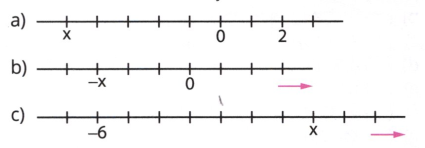
\includegraphics[width=1.1\linewidth]{6FMA79_imagens/imagem1}
			\item Calcule.
			\begin{enumerate}[a)]
				\item $|-8|$
				\item $|12 - 5|$
				\item $|4 - 6|$
				\item $-|-6 + 5|$
				\item $||2 - 7| - 9|$
			\end{enumerate}
   		\end{enumerate}
        $~$ \\ $~$ \\ $~$ \\ $~$ \\ $~$ \\ $~$ \\ $~$ \\ $~$ \\ $~$ \\ $~$ \\ $~$ \\ $~$ \\ $~$ \\ $~$ \\ $~$ \\ $~$ \\ $~$ \\ $~$ \\ $~$ \\ $~$ \\ $~$ \\ $~$ \\ $~$ \\ $~$ \\
        \end{multicols}
\end{document}